%%%%%%%%%%%%%%%%%%%%%%%%%%%%%%%%%%%%%%%%%%%%%%%%%%%%%%%%%%%%%%%%%%%%%%%%%%%%%%%%
% app_glossary.tex: Glossary Appendix:
%%%%%%%%%%%%%%%%%%%%%%%%%%%%%%%%%%%%%%%%%%%%%%%%%%%%%%%%%%%%%%%%%%%%%%%%%%%%%%%%
\chapter{Glossary and Acronyms}
\label{app_glossary}
%%%%%%%%%%%%%%%%%%%%%%%%%%%%%%%%%%%%%%%%%%%%%%%%%%%%%%%%%%%%%%%%%%%%%%%%%%%%%%%%
Care has been taken in this thesis to minimize the use of jargon and
acronyms, but this cannot always be achieved.  This appendix defines
jargon terms in a glossary, and contains a table of acronyms and their
meaning.
%%%%%%%%%%%%%%%%%%%%%%%%%%%%%%%%%%%%%%%%%%%%%%%%%%%%%%%%%%%%%%%%%%%%%%%%%%%%%%%%

%%%%%%%%%%%%%%%%%%%%%%%%%%%%%%%%%%%%%%%%%%%%%%%%%%%%%%%%%%%%%%%%%%%%%%%%%%%%%%%%
% Glossary {{{
%%%%%%%%%%%%%%%%%%%%%%%%%%%%%%%%%%%%%%%%%%%%%%%%%%%%%%%%%%%%%%%%%%%%%%%%%%%%%%%%
\section{Glossary}
\label{jargonapp}
%%%%%%%%%%%%%%%%%%%%%%%%%%%%%%%%%%%%%%%%%%%%%%%%%%%%%%%%%%%%%%%%%%%%%%%%%%%%%%%%
\begin{itemize}

\item \textbf{Cosmic-Ray Muon} (\textbf{CR $\mu$}) -- A muon coming from
the abundant energetic particles originating outside of the Earth's
atmosphere.
\item \textbf{SUSY} -- A theoretical model based on a fundamental symmetry called supersymmetry in which the fermions and bosons can exchange their spin, extending the standard model to account for the stability in the observed Higgs boson mass and to also predicting the existence of many extra new particles which could be candidates of dark matter.
\item \textbf{CMS Coordinate System} -- CMS uses a right-handed coordinate system, with the origin at the nominal interaction point, the \emph{$x$}-axis pointing to the center of the LHC, 
the \emph{$y$}-axis pointing up (perpendicular to the LHC plane), and the \emph{$z$}-axis along the counterclockwise-beam direction. The polar angle, $\theta$, 
is measured from the positive \emph{$z$}-axis and the azimuthal angle, $\phi$, is measured in the \emph{$x$-$y$} plane. 
\item \textbf{Eta}  -- 
\begin{equation}
\boldmath{\eta} = \boldmath{-\ln\tan(\theta/2)}
\end{equation}
\item \textbf{Transverse Energy and Momentum} -- The transverse energy and momentum are defined as
\begin{eqnarray}
 \boldmath{\ET} &= \boldmath{E\sin\theta} \\
 \boldmath{\PT} &= \boldmath{p\sin\theta} 
\end{eqnarray} 
 where $p$ is the momentum measured in the tracking system and $E$ is the energy measured in the calorimeters.
 
\item \textbf{Missing Transverse Energy} or \MET --
\begin{equation}
\boldmath{\MET} = \boldmath{\vert -\sum_{i}\ET^{i}\vec{n_{i}}\vert}
\end{equation}
 where $\vec{n_{i}}$ is a unit vector that points from the interaction vertex to the transverse plane.

\end{itemize}
%%%%%%%%%%%%%%%%%%%%%%%%%%%%%%%%%%%%%%%%%%%%%%%%%%%%%%%%%%%%%%%%%%%%%%%%%%%%%}}}

%%%%%%%%%%%%%%%%%%%%%%%%%%%%%%%%%%%%%%%%%%%%%%%%%%%%%%%%%%%%%%%%%%%%%%%%%%%%%%%%
% Acronyms {{{
%%%%%%%%%%%%%%%%%%%%%%%%%%%%%%%%%%%%%%%%%%%%%%%%%%%%%%%%%%%%%%%%%%%%%%%%%%%%%%%%
\section{Acronyms}
\label{acronymsec}
%%%%%%%%%%%%%%%%%%%%%%%%%%%%%%%%%%%%%%%%%%%%%%%%%%%%%%%%%%%%%%%%%%%%%%%%%%%%%%%%

%\setlength\LTleft{0pt}
%\setlength\LTright{0pt}

\begin{longtable}{|p{0.25\textwidth}|p{0.75\textwidth}|}
\caption{Acronyms} \label{Acronyms} \\

\hline
LLNP  & Long-Lived Neutral Particle. \\
DM    &  Dark Matter. \\
DE     &  Dark Energy. \\
SM   & Standard Model \\
BSM  & Beyond Standard Model \\
SUSY & Supersymmetry \\
GMSB   & Gauge Mediated Supersymmetry Breaking \\
LHC & Large Hadron Collider \\
CMS & Compact Muon Solenoid \\
DAQ & Data Acquisition Board \\
FPGA & Field Programmable Gate Arrays \\
ASIC & Application Specific Integrated Circuits \\

\hline \hline
\endfirsthead

\multicolumn{2}{l}%
{{\bfseries \tablename\ \thetable{} -- continued from previous page}} \\
\hline
Acronym & Meaning \\
\hline \hline
\endhead

\hline \hline \multicolumn{2}{|r|}{{Continued on next page}} \\ \hline
\endfoot

\hline \hline
\endlastfoot

CR$\mu$ & Cosmic-Ray Muon \\

\end{longtable}


%%%%%%%%%%%%%%%%%%%%%%%%%%%%%%%%%%%%%%%%%%%%%%%%%%%%%%%%%%%%%%%%%%%%%%%%%%%%%%%%
\section{Analysis How To and Data Samples}
\subsection{Check Out Software Packages}
To check out the analysis packages, do the following steps:
\begin{itemize}
\item \texttt{cmsrel CMSSW\_5\_3\_29} 
\item \texttt{cd CMSSW\_5\_3\_29\char`\\src} 
\item \texttt{git clone git@github.com:sckao/DPAnalysis.git}
\item \texttt{git clone git@github.com:TENorbert/UncleanedGSFElectron.git}
\item \texttt{git@github.com:TENorbert/GMSB\-8\-TeV.git}
\item \texttt{git@github.com:TENorbert/DPAnalysis\_Limit\_Setting\_Tools.git}
\item \texttt{scram b \-j9}

\end{itemize}

\subsection{Data Samples}
In Table \ref{tab:DATA} show the data samples and the corresponding integrated luminosity.
\newline
The \textit{jason} file with the list of certified good luminosity sections is 
\newline
 \textbf{Cert\_8TeVPromptReco\_Colllisions12\_JASON.txt}.

\vspace{5mm}
\begin{minipage}{0.90\linewidth}  
\begin{center}
%\begin{table}[ht]
%\renewcommand\arraystretch{1.2}
\begin{tabular}{l l}
\toprule
\hline
\bfseries{Data Sample} & \vtop{\hbox{\strut{\bfseries{Recorded Luminosity}}}  \hbox{\strut{ $[\fbinv]$ }}} \\
\hline
\toprule
 \vtop{\hbox{\strut{\texttt{/Run2012B/SinglePhoton/}}}
 \hbox{\strut{\texttt{EXODisplacedPhoton-PromptSkim-v3}}}} & 5.1 \\
 \hline
 \vtop{\hbox{\strut{\texttt{/Run2012C/SinglePhoton/}}}
 \hbox{\strut{\texttt{EXODisplacedPhoton-PromptSkim-v3 }}}} & 6.9 \\
 \hline
 \vtop{\hbox{\strut{\texttt{/Run2012D/SinglePhoton/}}}
 \hbox{\strut{\texttt{EXODisplacedPhoton-PromptSkim-v3 }}}} & 7.1 \\
\hline\hline
\texttt{/SingleElectron/Run2012A-22Jan2013-v1/AOD} & 5.2 \\
\texttt{/DoubleElectron/Run2012C-22Jan2013-v1/AOD} & 4.8 \\
\hline
\bottomrule
\end{tabular}
\captionof{table}{Data samples and their corresponding integrated luminosity totaling 19.1~\fbinv used in the our delayed photon search analysis}
\label{tab:DATA}
%\end{table}
\end{center}
\end{minipage}

\subsection{Event Display}
\paragraph{Event Properties:}
The one event observed in our signal region has a final state: a photon, 2 jets and large MET.
\newline
PHOTON: \pt = 225 \GeVcc, ECAL Time = 12\ns, $\eta = 0.32$ and $\phi = 1.13$ \newline
MET: $\ETslash\hspace{0.15cm} = 333\GeV$,  ${\ETslash}^{\gamma}\hspace{0.15cm} = 125 \GeV$ \newline
JETS: Jet1 $\pt = 86\GeVc$ and Jet2 $\pt = 36\GeVc$

\vspace{5mm}
\begin{minipage}{0.95\linewidth} 
\begin{center}
%\mbox{
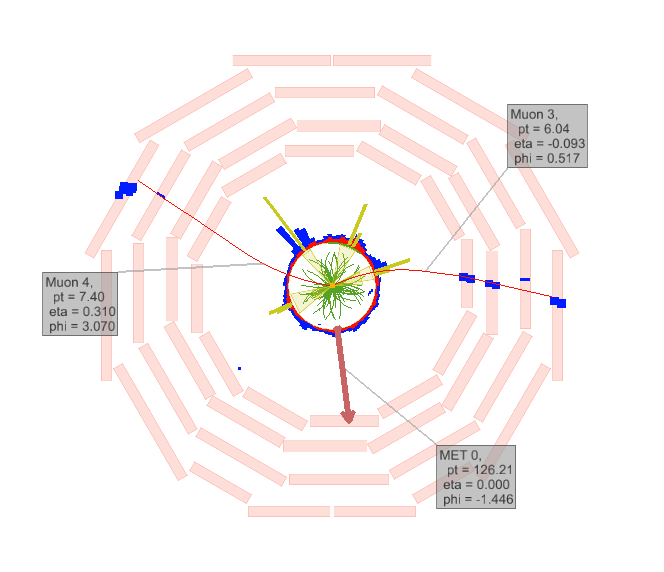
\includegraphics[height=10cm, width=0.9\textwidth]{THESISPLOTS/Observed_Event_CMS_Run206484-Lumi620-EventNumber871295869-206484_871295869_620_RhoPhi.png}
\captionof{figure}{$\rho-\phi$-view of the observed event in CMS detector.}
\label{fig:RHO-PHI}
\end{center}
\end{minipage}

\vspace{5mm}

\begin{minipage}{0.90\linewidth} 
\begin{center}
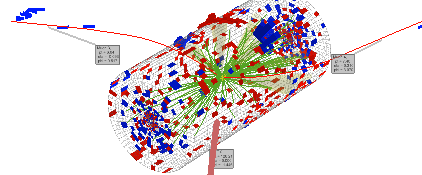
\includegraphics[height=7cm, width=0.8\textwidth]{THESISPLOTS/Observed_Event_CMS_Run206484-Lumi620-EventNumber871295869-206484_871295869_620_3DTower.png} 
%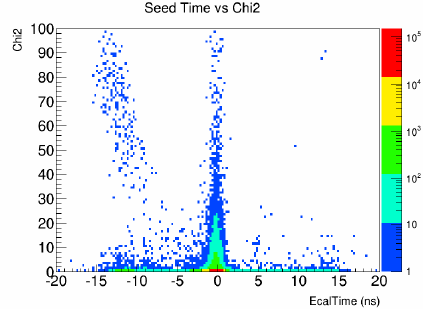
\includegraphics[height=6cm, width=0.5\textwidth]{THESISPLOTS/Seed-Time-Chi2.png}
\captionof{figure}{3-D view of the observed event in CMS detector.}
\label{fig:3-D}
\end{center}
\end{minipage}

%%%%%%%%%%%%%%%%%%%%%%%%%%%%%%%%%%%%%%%%%%%%%%%%%%%%%%%%%%%%%%%%%%%%%%%%%%%%%}}}
